% ============================================================
% physio-placebo — living supervisor report
% Figures:  python scripts/plot_supervisor_report.py
% Compile:  tectonic reports/supervisor_master_report.tex
% Share:    reports/supervisor_master_report.pdf
%
% UPDATE RULE (every closed week):
%   1. Bump \ReportDate and the header "through Week N".
%   2. Append one row to the Revision log.
%   3. Tick the snapshot table; add numbers only for closed weeks.
%   4. Do not write results into weeks that are not tagged done.
%   5. Do not edit the filed OSF Models text.
%   6. Do not put process notes in the PDF (how we update this file,
%      "I will not start week N until you say so"). Those stay internal.
% ============================================================
\documentclass[11pt]{article}

\usepackage[a4paper,margin=1in]{geometry}
\usepackage{iftex}
\ifPDFTeX
  \usepackage[T1]{fontenc}
  \usepackage[utf8]{inputenc}
  \usepackage{lmodern}
\else
  \usepackage{fontspec}
\fi
\usepackage{microtype}
\usepackage{amsmath}
\usepackage{booktabs}
\usepackage{colortbl}
\usepackage{array}
\usepackage{tabularx}
\usepackage{ragged2e}
\usepackage{xcolor}
\usepackage{titlesec}
\usepackage{fancyhdr}
\usepackage{lastpage}
\usepackage{enumitem}
\usepackage{graphicx}
\graphicspath{{figures/}{reports/figures/}}
\usepackage{caption}
\renewcommand{\topfraction}{0.92}
\renewcommand{\bottomfraction}{0.72}
\renewcommand{\textfraction}{0.08}
\renewcommand{\floatpagefraction}{0.75}
\setcounter{topnumber}{3}
\setcounter{totalnumber}{5}
\setlength{\textfloatsep}{8pt plus 2pt minus 2pt}
\setlength{\intextsep}{8pt plus 2pt minus 2pt}
\usepackage[hidelinks]{hyperref}
\captionsetup{
  font=small,
  labelfont={bf,color=Accent},
  textfont={color=AccentSoft},
  skip=4pt,
}

\definecolor{Accent}{HTML}{0F4C5C}
\definecolor{AccentSoft}{HTML}{1B6B7A}
\definecolor{RuleGray}{HTML}{B8C4C8}
\definecolor{TableHead}{HTML}{E8F1F3}
\definecolor{Ask}{HTML}{7A2E0E}
\definecolor{Ok}{HTML}{1F6B4A}
\definecolor{Muted}{HTML}{5C6B70}

\newcommand{\ReportDate}{14 October 2026}
\newcommand{\ReportThrough}{Week 8}
\newcommand{\ReportNext}{Week 9 (verbalizer ablation) --- not started}

\hypersetup{
  pdftitle={physio-placebo: living supervisor report (through Week 8)},
  pdfauthor={Shrijak Kumar},
  pdfsubject={Independent study living report},
  linkcolor=Accent,
  urlcolor=AccentSoft,
}

\titleformat{\section}
  {\large\bfseries\color{Accent}}
  {\thesection}{0.7em}{}
\titlespacing*{\section}{0pt}{1.15em}{0.4em}
\titleformat{\subsection}
  {\normalsize\bfseries\color{AccentSoft}}
  {\thesubsection}{0.6em}{}
\titlespacing*{\subsection}{0pt}{0.9em}{0.3em}

\pagestyle{fancy}
\fancyhf{}
\renewcommand{\headrulewidth}{0.4pt}
\renewcommand{\footrulewidth}{0.3pt}
\fancyhead[L]{\small\color{AccentSoft} physio-placebo}
\fancyhead[R]{\small\color{AccentSoft} living report \textbullet\ through \ReportThrough}
\fancyfoot[L]{\small\color{Muted} Shrijak Kumar \textbullet\ Dr.\ Siddharth}
\fancyfoot[R]{\small\color{Muted} \thepage\ / \pageref{LastPage}}
\fancyfoot[C]{}

\arrayrulecolor{Accent!55}
\setlength{\parindent}{0pt}
\setlength{\parskip}{0.48em}
\linespread{1.05}
\setlength{\emergencystretch}{2em}
\setlist[itemize]{leftmargin=1.2em,itemsep=0.15em,topsep=0.25em}
\setlist[enumerate]{leftmargin=1.2em,itemsep=0.15em,topsep=0.25em}
\newcolumntype{L}[1]{>{\RaggedRight\arraybackslash}p{#1}}
\newcolumntype{C}[1]{>{\centering\arraybackslash}p{#1}}
\newcolumntype{Y}{>{\RaggedRight\arraybackslash}X}

\begin{document}

{\large\scshape\color{AccentSoft} Independent study --- living supervisor report\par}
\vspace{0.35em}
{\color{Accent}\hrule height 1.15pt}
\vspace{0.65em}
{\LARGE\bfseries\color{Accent} physio-placebo\par}
\vspace{0.2em}
{\large Is the LLM reading the signal, or is the verbalizer doing the classifying?\par}
\vspace{0.55em}
{\color{Accent}\hrule height 1.15pt}
\vspace{0.75em}

\begin{tabular}{@{}L{3.5cm}L{12.0cm}@{}}
\textbf{Student} & Shrijak Kumar \\
\textbf{Advisor} & Dr.\ Siddharth, Plaksha University \\
\textbf{This edition} & \ReportDate \\
\textbf{Closed through} & \ReportThrough \quad (git tags \texttt{week-01-done} \ldots\ \texttt{week-06-done}) \\
\textbf{Next block} & \ReportNext \\
\textbf{Repository} & \url{https://github.com/shrijacked/physio-placebo} \\
\textbf{Pre-registration} & \url{https://osf.io/62r5t} \quad DOI 10.17605/OSF.IO/62R5T \\
\end{tabular}

\vspace{0.15em}
{\small\color{Muted}
This is the document I will keep sending. Each time a week is tagged done, I add that week's
real numbers and leave later weeks blank. Nothing here changes the filed OSF text.
\par}

\section{Revision log}

\begin{center}
{\small
\begin{tabularx}{\textwidth}{@{}L{3.1cm}L{2.6cm}Y@{}}
\rowcolor{TableHead}
\textbf{Edition} & \textbf{Closed through} & \textbf{What this PDF added} \\
\midrule
21 Sep 2026 & Week 6 & First living edition. Weeks 1--6 numbers, A/B/C tables, methods sketch, SDS, input examples. \\
11 Oct 2026 & Week 6 & Health-LLM comparison arm. Prompting and fine-tuning are separate tables. Weeks 7--8 are still not started. \\
14 Oct 2026 & Week 8 & Surrogate ladder and classical ledger. 120 model cells, raw logprobs saved. Week 9 not started. \\
\bottomrule
\end{tabularx}
}
\end{center}

\section{Snapshot}

\begin{center}
{\small
\begin{tabularx}{\textwidth}{@{}L{3.3cm}L{2.6cm}Y@{}}
\rowcolor{TableHead}
\textbf{Block} & \textbf{State} & \textbf{One-line result} \\
\midrule
Week 1 --- data & Closed 16 Sep & WESAD 15/15, MAUS 22/22, CogWear 10/11; 0 feature-NaN drops \\
Week 2 --- floors & Closed 16 Sep & WESAD strong (logreg 0.918); MAUS and CogWear weak \\
Week 3 --- anchor + OSF & Closed 20 Sep & MedAlpaca MAE $2.689\pm 0.038$ vs paper $0.76\pm 0.1$ \\
Weeks 4--5 --- A/B & Closed 21 Sep & Best LLM cell: Qwen WESAD A bin-mean 0.595 [0.550, 0.647] \\
Week 6 --- plots (C) & Closed 21 Sep & Qwen2.5-VL at chance on WESAD and MAUS \\
Comparison arm & Added 11 Oct & PMData stress MAE only. Separate from the WESAD grid. \\
Weeks 7--8 --- surrogates & Closed 14 Oct & 120 cells scored. WESAD logreg stays high on IAAFT (0.880) and on the label-preserving permutation (0.954). \\
Week 9 --- verbalizer & Not started & Neutralize / mis-sign adjectives (the paper's core) \\
Week 10 --- SDS card & Not started & Protected mid-semester result \\
\bottomrule
\end{tabularx}
}
\end{center}

{\color{Ok}\textbf{What I would like you to take from this edition.}}
Real-signal prompting is in. Classical WESAD is still far above every LLM cell. Paradigm~C
(plots) is at chance, which is the direction we pre-registered. The next scientific step is
the surrogate ladder, not more prompt tuning.

\section{The study, in one paragraph}

Published wearable-LLM papers report that language models can infer stress or workload from
sensor text. They almost never test whether that accuracy depends on the physiological signal.
This study runs the same class of prompts on WESAD, MAUS, and CogWear under strict
leave-one-subject-out, then replaces the recording with a ladder of surrogates and measures
how much accuracy survives. The intellectual core is a verbalizer ablation: do models read
the numbers, or the class-suggestive adjectives in the template? A negative result is
pre-registered as publishable.

Scoring is locked: one forward pass, argmax over the log-probabilities of label tokens
\texttt{A}/\texttt{B}. No free generation. Prompt IDs are chosen on two held-out subjects
per dataset (seed 1337) and then frozen before any surrogate run.

The pre-registered Surrogate Dependence Score is
\begin{equation*}
\mathrm{SDS}
=
\frac{M_{\mathrm{real}}-M_{\mathrm{surrogate}}}{M_{\mathrm{real}}-M_{\mathrm{chance}}},
\end{equation*}
with $M$ the pooled LOSO macro-F1 and $M_{\mathrm{chance}}$ the permutation-floor mean.
If a cell's real-signal margin over that floor has a bootstrap CI that includes zero,
SDS is undefined and only the raw delta is reported.

\begin{figure}[!ht]
\centering
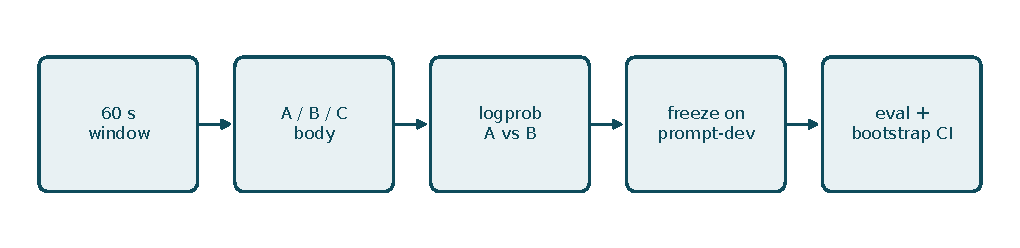
\includegraphics[width=\textwidth]{figures/fig_methods.pdf}
\caption{One cell. A 60\,s window becomes an A, B, or C body; the scorer takes
$\arg\max$ of $P(\texttt{A})$ and $P(\texttt{B})$. Prompt IDs freeze on two
prompt-dev subjects. Reported numbers are eval subjects only.}
\end{figure}

{\small
The same WESAD 60\,s ECG window in the three locked forms.
A is bin-mean ($n{=}128$), the winning WESAD A cell.
B is verbalizer~(i); four of eighteen feature sentences (the adjective leak is
intentional and is the Week~9 ablation).
C is the matplotlib PNG the VL model receives. Subject id and class are not on the plot.
\par}
\noindent\textit{Numbers --- the ECG averaged into 128 bins}
\begin{quote}\ttfamily\footnotesize
ecg fs=700 Hz n=128 scheme=bin\_mean:\\0.04024 0.005173 -0.01352 -0.01912 0.03245 -0.00422 -0.02569 0.0196\\... 117 values omitted ...\\-0.04705 -0.00251 -0.06615
\end{quote}
\noindent\textit{Sentences --- 4 of the 18 feature lines}
\begin{quote}\ttfamily\footnotesize
eda\_tonic\_mean is reduced (0.7358), calmer-typical.\\hrv\_mean\_hr is elevated (89.28), stress-typical.\\hrv\_sdnn is reduced (41.18), stress-typical.\\hrv\_rmssd is reduced (17.7), stress-typical.
\end{quote}

\begin{figure}[!ht]
\centering
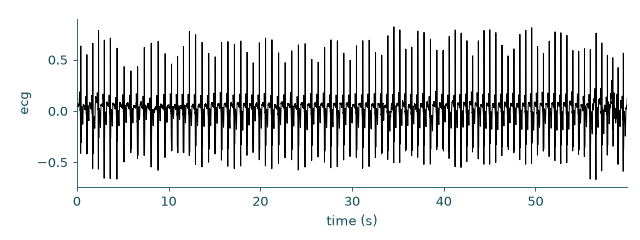
\includegraphics[width=0.86\textwidth]{figures/fig_input_c.png}
\caption{Paradigm C view of that same window. No subject id and no class name.}
\end{figure}

\section{Week 1 --- data and harness}

Windows are 60\,s with a 30\,s stride, cut strictly inside one protocol segment.

\begin{center}
{\small
\begin{tabular}{@{}lcccc@{}}
\toprule
\rowcolor{TableHead}
\textbf{Dataset} & \textbf{Subjects} & \textbf{Windows} & \textbf{Class split} & \textbf{NaN drops} \\
\midrule
WESAD & 15 / 15 & 1{,}042 & 731 non-stress / 311 stress & 0 \\
MAUS & 22 / 22 & 1{,}086 & 362 low / 724 high & 0 \\
CogWear & 10 / 11 & 114 & 39 baseline / 75 Stroop & 0 \\
\bottomrule
\end{tabular}
}
\end{center}

CogWear subject~3 is excluded because PhysioNet is missing that subject's EDA file (logged
in the prereg). Feature code is hash-locked (NeuroKit2 0.2.13). LOSO and a prompt-dev split
are tested. SensorLM captioning templates are vendored (Apache-2.0) for a later optional
verbalizer variant; they are not a model-under-test.

\section{Week 2 --- classical floor}

Locked \emph{before} any LLM grid run, on byte-identical feature matrices (seed 1337;
1{,}000 within-subject label permutations). These are the numbers an LLM cell must beat.

\begin{center}
{\small
\begin{tabular}{@{}lccccc@{}}
\toprule
\rowcolor{TableHead}
\textbf{Dataset} & \textbf{Logreg L2} & \textbf{Depth-3 tree} & \textbf{Majority} & \textbf{Perm.\ p95} & \textbf{Signal} \\
\midrule
WESAD ($n{=}15$) & 0.918 & 0.848 & 0.412 & 0.433 & Strong \\
MAUS ($n{=}22$) & 0.444 & 0.482 & 0.400 & 0.413 & Weak \\
CogWear ($n{=}10$) & 0.569 & 0.560 & 0.397 & 0.541 & Weak \\
\bottomrule
\end{tabular}
}
\end{center}

WESAD is the dataset that can actually test signal dependence. MAUS and CogWear barely
clear (or fail) the permutation floor; many of those cells will hit the pre-registered SDS
validity gate. We will then report raw deltas, not a ratio on a near-zero denominator.

\begin{figure}[!ht]
\centering
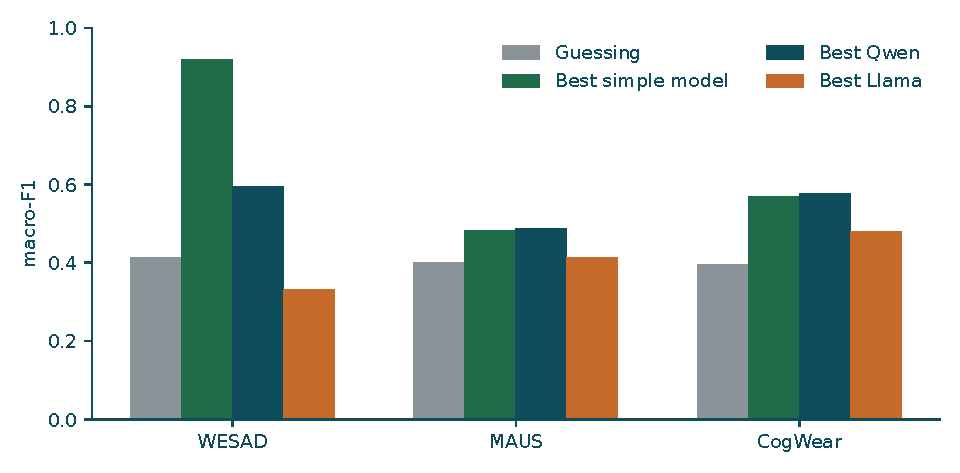
\includegraphics[width=\textwidth,height=2.15in,keepaspectratio]{figures/fig_floors_vs_llm.pdf}
\caption{Locked classical floor versus the best real-signal A/B cell per model.
WESAD is the only dataset where a classical model is far above majority.
Every LLM bar is the best of that model's three A/B cells.}
\end{figure}

\section{Week 3 --- fidelity anchor and OSF}

OSF registration is public (\url{https://osf.io/62r5t}). Predictions on file:
\begin{itemize}
  \item SDS ${<}\,0.3$ for raw-series and plot paradigms;
  \item verbalized features lose ${>}\,50\%$ of their above-chance margin when adjectives are neutralized;
  \item adversarially mis-signed adjectives flip ${>}\,40\%$ of items.
\end{itemize}

Fidelity anchor (Health-LLM PMData stress, zero-shot MedAlpaca-7b) on the HTI RTX A6000
(20 Sep 2026): MAE $\mathbf{2.689 \pm 0.038}$ versus paper $0.76 \pm 0.1$ (gap $+1.929$;
6/897 parse failures). Completions are mostly ``out of 5 / out of 10''; the locked
first-number scorer reads 5 or 10. I am \emph{not} retuning that scorer --- the gap is the
result. The 299-item eval split and the three prompt hashes were locked before the run.

\begin{figure}[!ht]
\centering
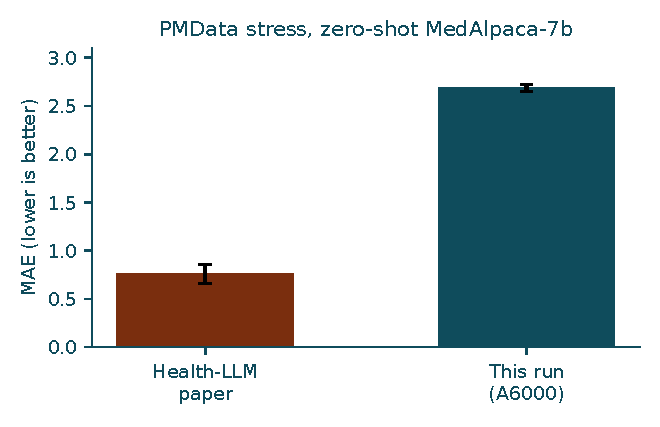
\includegraphics[width=0.58\textwidth]{figures/fig_anchor_mae.pdf}
\caption{Health-LLM Table~3 cell (paper $0.76\pm 0.1$) versus the locked first-number
reproduction on the HTI A6000 ($2.689\pm 0.038$).}
\end{figure}

Executed models (public OSF update, 20 Sep 2026) are Qwen3-8B, Llama-3.1-8B-Instruct, and
Qwen2.5-VL-7B-Instruct via vLLM in fp16. The filed Models section still names gpt-4.1;
that is a disclosed post-registration deviation (OpenAI 50 req/day cap). I am not rewriting
the frozen OSF Models paragraph.

\section{Weeks 4--5 --- Paradigms A and B}

Prompt-dev subjects (excluded from eval): WESAD S2/S8, MAUS 015/023, CogWear 4/8.
Scoring failures: 0 / 11{,}916 eval windows. CIs are subject-bootstrap, 1{,}000 resamples,
seed 1337.

\begin{center}
{\small
\begin{tabular}{@{}llcc@{}}
\toprule
\rowcolor{TableHead}
\textbf{Dataset} & \textbf{Cell} & \textbf{Qwen3-8B} & \textbf{Llama-3.1-8B} \\
\midrule
WESAD & A stride & 0.427 [0.392, 0.465] & 0.333 [0.301, 0.370] \\
WESAD & A bin-mean & \textbf{0.595 [0.550, 0.647]} & 0.230 [0.227, 0.233] \\
WESAD & B verbalizer & 0.584 [0.462, 0.699] & 0.283 [0.247, 0.324] \\
MAUS & A stride & 0.467 [0.436, 0.499] & 0.413 [0.403, 0.426] \\
MAUS & A bin-mean & 0.483 [0.452, 0.516] & 0.400 [0.400, 0.400] \\
MAUS & B verbalizer & 0.487 [0.439, 0.531] & 0.400 [0.400, 0.400] \\
CogWear & A stride & 0.576 [0.443, 0.689] & 0.404 [0.392, 0.417] \\
CogWear & A bin-mean & 0.396 [0.380, 0.411] & 0.440 [0.399, 0.495] \\
CogWear & B verbalizer & 0.475 [0.393, 0.504] & 0.479 [0.375, 0.640] \\
\bottomrule
\end{tabular}
}
\end{center}

Winning prompts differ by cell (frozen in \texttt{configs/frozen\_prompts.lock.yaml}).
The bold cell is Qwen, WESAD, Paradigm~A, bin-mean, clinical 0-shot --- the only LLM
number that clearly clears WESAD majority (0.412). It is still far below the classical
logreg floor (0.918). Llama's two MAUS cells at $0.400\pm 0$ are constant-class on every
eval subject, not a crash. CogWear CIs are wide ($n{=}90$ eval windows).

\begin{figure}[!ht]
\centering
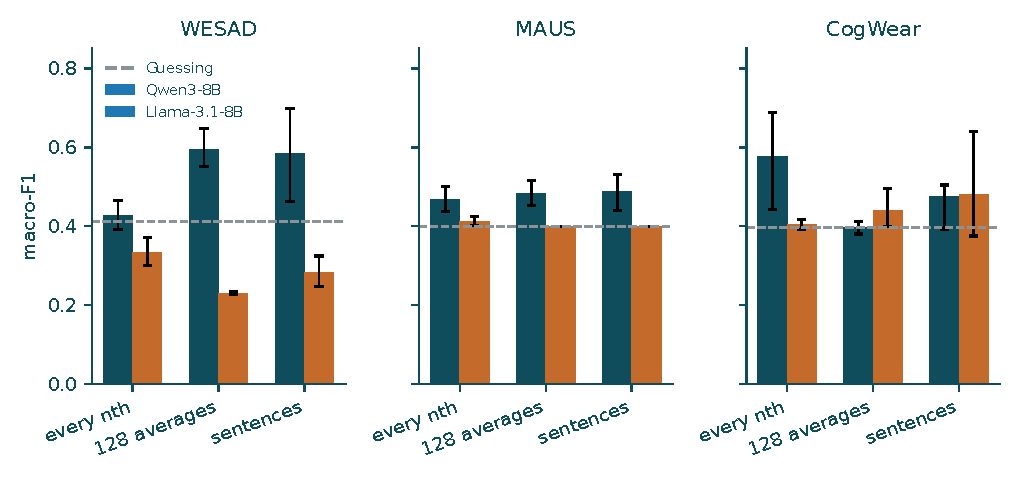
\includegraphics[width=\textwidth,height=2.2in,keepaspectratio]{figures/fig_ab_grid.pdf}
\caption{Real-signal Paradigms A and B, eval subjects only, subject-bootstrap 95\% CIs.
Dashed line is majority-class macro-F1. Qwen is above Llama on WESAD and MAUS.
The WESAD A bin-mean cell is the only LLM number that clearly clears WESAD majority.}
\end{figure}

\section{Week 6 --- Paradigm C (plots)}

Qwen2.5-VL-7B-Instruct, matplotlib line plot of the primary channel (WESAD ECG, MAUS PPG).
Same window $\rightarrow$ same PNG bytes. No subject id and no class name on the figure.
CogWear has no C cell. Frozen prompt: instruction 4-shot.

\begin{center}
{\small
\begin{tabular}{@{}lccc@{}}
\toprule
\rowcolor{TableHead}
\textbf{Dataset} & \textbf{Prompt} & \textbf{macro-F1 [95\% CI]} & \textbf{Windows} \\
\midrule
WESAD & instruction 4-shot & 0.412 [0.410, 0.414] & 906 \\
MAUS & instruction 4-shot & 0.400 [0.399, 0.400] & 990 \\
\bottomrule
\end{tabular}
}
\end{center}

Both sit on chance. The tight CIs mean the model is almost always emitting one class.
That is consistent with pre-registered prediction~1 (plot paradigm should not carry
signal). I am not retuning C prompts.

\begin{figure}[!ht]
\centering
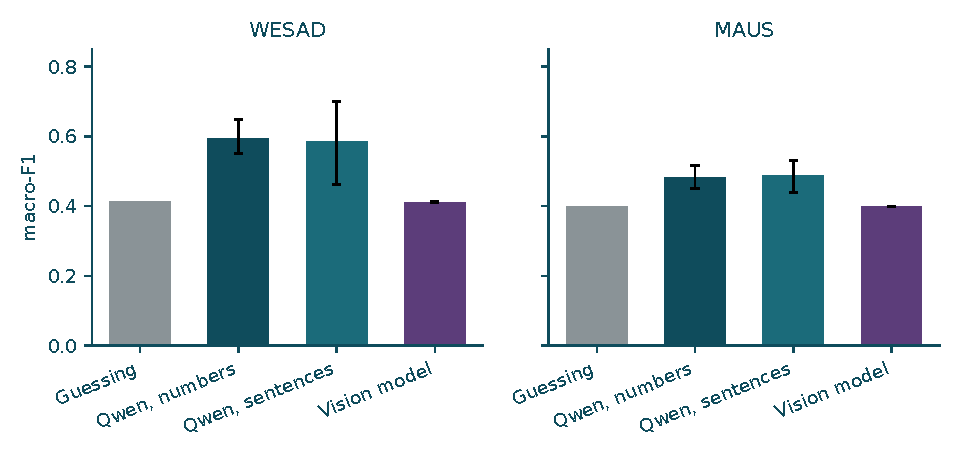
\includegraphics[width=\textwidth,height=2.15in,keepaspectratio]{figures/fig_paradigm_c.pdf}
\caption{Paradigm C against majority and the same model's A/B cells.
Qwen2.5-VL sits on chance on both WESAD and MAUS.}
\end{figure}

\section{What is next (not started)}

\begin{enumerate}
  \item \textbf{Week 9.} Verbalizer ablation on Paradigm~B: original / neutralized /
        mis-signed adjectives. SensorLM templates remain a pending yes/no from you
        (variant~iv).
  \item \textbf{Week 10.} SDS report card. Protected. If the calendar slips, we cut
        stretch work, not this.
\end{enumerate}

\section{Comparison arm --- Health-LLM, PMData stress}

This is not a new week. WESAD, MAUS, and CogWear macro-F1 stay in the tables above.
The match is Kim et al., Health-LLM, CHIL 2024, PMData stress, MAE.
Train rows are the released pool minus one sensor string that also appears in the
locked 299-item eval (653 left). The paper's 10\% test split is not claimed to be
that eval. Recipe lock: \texttt{configs/healthllm\_finetune.lock.yaml}.

\begin{center}
{\small
\begin{tabular}{@{}llcc@{}}
\toprule
\rowcolor{TableHead}
\textbf{Row} & \textbf{Model} & \textbf{Adaptation} & \textbf{MAE} \\
\midrule
Paper Table 3 & MedAlpaca-7b & zero-shot & $0.76 \pm 0.1$ \\
Locked rerun & MedAlpaca-7b & zero-shot & $2.689 \pm 0.038$ \\
Different backbone & Qwen3-8B & zero-shot, same prompts & $0.795 \pm 0.020$ \\
Different backbone & Llama-3.1-8B-Instruct & zero-shot, same prompts & $2654 \pm 43$ \\
\bottomrule
\end{tabular}}
\end{center}

\noindent Qwen answers \texttt{Answer: 3}. Llama writes Python that pastes step counts;
the locked first-number scorer reads those counts. The scorer was not changed.
Always answering 3 on this eval has MAE 0.401, which is still below Qwen.

\begin{center}
{\small
\begin{tabular}{@{}llcc@{}}
\toprule
\rowcolor{TableHead}
\textbf{Row} & \textbf{Model} & \textbf{Adaptation} & \textbf{MAE} \\
\midrule
Paper Table 4 & MedAlpaca-7b & fine-tuned on PMData & 0.38 \\
This arm, eval seed 0 & MedAlpaca-7b LoRA & 3 epochs, batch 128, fp16 & 2.697 \\
\bottomrule
\end{tabular}}
\end{center}

\noindent 297 of 299 fine-tune completions parsed. They are still ``out of 5'', so the
scorer reads 5. The same model's zero-shot seed 0 on this eval was 2.714. The LoRA
run did not move that cell. Deviations from the paper (no oversampling, warmup 0
because this pool is 653 rows, per-device batch 1) are in the lock file.

\section{Weeks 7--8 --- surrogate ladder}

Every frozen prompt was scored again after the window was replaced.
120 cells, 0 scoring failures. Each row in
\texttt{results/surrogates/eval/} keeps the label-token logprobs.
The label-preserving permutation is reported and is not a null.

Classical logistic regression on the surrogate features
(\texttt{results/surrogates/ledger/20261013T193152Z/ledger.json}):

\begin{center}
{\small
\begin{tabular}{@{}lccc@{}}
\toprule
\rowcolor{TableHead}
\textbf{Surrogate} & \textbf{WESAD} & \textbf{MAUS} & \textbf{CogWear} \\
\midrule
Gaussian & 0.412 & 0.400 & 0.486 \\
IAAFT & 0.880 & 0.405 & 0.458 \\
Wrong subject, label broken & 0.411 & 0.405 & 0.380 \\
Flatline & 0.412 & --- & 0.397 \\
Signal deleted & --- & --- & --- \\
Wrong subject, label kept & 0.954 & 0.494 & 0.773 \\
\bottomrule
\end{tabular}}
\end{center}

\noindent A dash means the features were absent or entirely missing, so the
regression was not fit. On WESAD the phase-randomized series still carries
class information (0.880), and keeping the condition while swapping the person
carries still more (0.954). Gaussian noise, a broken label, and a flat line
sit on the majority floor (0.412). SDS is Week 10. It is not computed here.

\section{Open items for you}

{\color{Ask}\textbf{Still useful from you.}}
SensorLM verbalizer variant~(iv): yes or no. Code is vendored; extra compute is near
zero. A decision lets me freeze the Week~9 ablation set.

GPU access is resolved (HTI A6000, account \texttt{shrijak}). The surrogate grid
already ran there.

\vspace{0.85em}
{\color{Accent}\hrule height 0.6pt}
\vspace{0.4em}
{\small\color{AccentSoft}
Shrijak Kumar \textbullet\ \ReportDate \textbullet\
Working log: \texttt{PROGRESS.md} \textbullet\
This report does not change the filed OSF text.\par}

\end{document}
